\documentclass[12pt]{article}

\usepackage{graphicx}
\usepackage{paralist}
\usepackage{listings}
\usepackage{booktabs}
\usepackage{hyperref}
\usepackage{subfig}
\usepackage{float}
\usepackage{mathtools}
\usepackage{fancyvrb}

\lstset{
basicstyle=\small\ttfamily,
columns=flexible,
breaklines=true
}
\DeclarePairedDelimiter\ceil{\lceil}{\rceil}
\DeclarePairedDelimiter\floor{\lfloor}{\rfloor}
\oddsidemargin 0mm
\evensidemargin 0mm
\textwidth 160mm
\textheight 200mm

\pagestyle {plain}
\pagenumbering{arabic}

\newcounter{stepnum}

\title{CS/SE 2XB3 Lab 7 Report\\Enrolled in CSL02}
\author{
  Wang, Mingzhe\\400316660\\
  \texttt{wangm235@mcmaster.ca}
  \and
  Li, Xing\\400292346\\
  \texttt{li64@mcmaster.ca}
  \and
  Moon, Hyosik\\400295620\\
  \texttt{moonh8@mcmaster.ca}
  }
\date{\today}



\begin{document}

\maketitle

\tableofcontents
\newpage

\section{Basic Graph Algorithms}
We implemented all relevant codes in \verb|graphs.py| file.

\bigskip

\section{Cycles and Connected Probability}

\subsection{Cycle test}
To randomly construct graphs with $k$ nodes and $c$ edges, we treat each edge as the combination of two different nodes, then use \verb|random.sample| function to choose c edges. The detail for this implementation can be found in \verb|cons_random_graph| of \verb|code.py|.\\\\
We designed the cycle test by increasing the number of edges from 1 to 400 for graphs with 100 nodes. For each number of edges $c$, we randomly generate 200 graphs, then calculated the portion of  graphs which have a cycle vs c.\\

\noindent
The observation is listed below:
\begin{itemize}
\item The test result (Figure \ref{graph_test}) shows that the portion of graphs which have a cycle increases as the edge number c increases, and when the edge number c is around 80, the portion almost converges to 1. 
\item In addition, the average value of c which roughly half the graphs to contain a cycle is 55.0, with the accepted value for ``half" is set as $(0.45, 0.55)$.
\end{itemize}

\begin{figure}[hbt!]
  \centering
  \includegraphics[width=0.5\textwidth]{Figures/graph_test.png}
  \caption{Cycles and Connected Probability test}
   \label{graph_test}
\end{figure}

\subsection{Connection test}
Following the same process, we also provide the connection test result in Figure \ref{graph_test}.\\

\noindent
The observation is listed below: 
\begin{itemize}
\item The portion of graphs which are connected increases as the edge number c increases, and when the edge number c is around 400, the portion almost converges to 1, (around 0.96). 
\item In addition, the average value of c which roughly half the graphs to be connected is 242.75, with the accepted value for ``half" is set as $(0.45, 0.55)$. 
\end{itemize}

\subsection{Why portion of connected graph is less than that of cyclic graph}
The portion of connected graphs needs a higher number of edges to reach the same portion of cyclic graphs. Because in the case of cycle, it requires at least (k-1) edges for a graph with k nodes to be connected; while in the case of cycle, a graph with k nodes can easily be cyclic even with only 3 edges. (Assume $k \geq 3$.) That's the reason that the portion of cyclic graphs starts to rise at about 3 and the portion of connected graph rises only after 150.

% ~\newline\noindent The curve is famous S-curve $1/(1+e^{-x})$. In statistics, it's cumulative distribution. In logistic regression and deep learning it is sigmoid function. In investment, it's business growth, and we need to invest when less than 20\% people realize the value of the business.


% \begin{figure}[hbt!]
%   \centering
%   \subfloat[Height of insertion (10,000(n), 50times)]{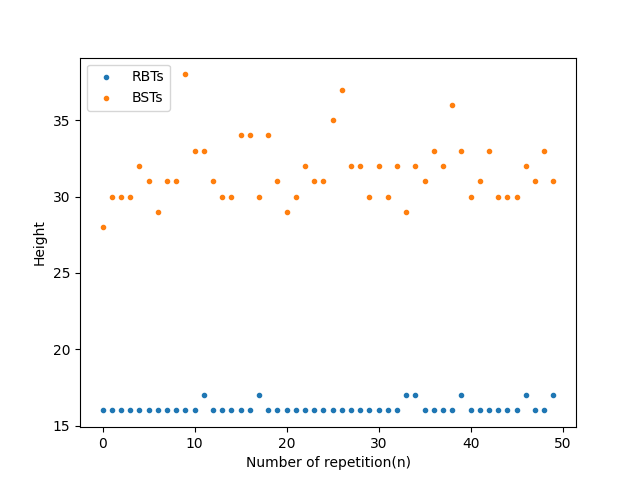
\includegraphics[width=0.49\textwidth]{Figures/rbt_bst_avg_10000.png}\label{r4}}
%   \hfill
%   \subfloat[Height of insertion (50,000(n), 10times)]{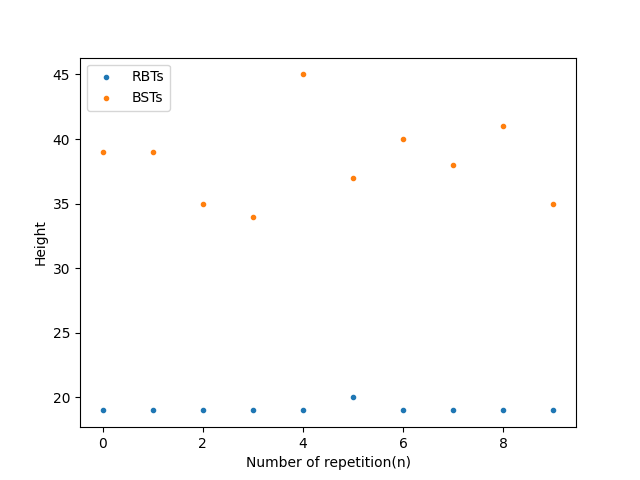
\includegraphics[width=0.49\textwidth]{Figures/rbt_bst_avg_50000.png}\label{r5}}
%   \caption{Red Black Tree insert result}
% \end{figure}

\newpage

\begin{thebibliography}{9}
% \bibitem{codesdope} 
% Red Black Tree,\\
% \texttt{https://www.codesdope.com/course/data-structures-red-black-trees-insertion/}

% \bibitem{wikipedia} 
% Binary heap,\\
% \texttt{https://en.wikipedia.org/wiki/Binary\_heap}

% \bibitem{wikipedia2} 
% k-ary heap,\\
% \texttt{https://en.wikipedia.org/wiki/D-ary\_heap}

% \bibitem{Geeks}
% m-ary tree,\\
% \texttt{https://www.quora.com/What-are-advantages-of-using-a-d-ary-tree-instead\\-of-a-binary-tree}

\end{thebibliography}

\end{document}
